% ============================================================
% Template de TCC (Artigo Científico) — Faculdade UCL
% Compile com pdfLaTeX + BibTeX (não depende de fontspec/XeLaTeX).
% ============================================================
\documentclass[12pt,a4paper]{article}

\usepackage[T1]{fontenc}
\usepackage[utf8]{inputenc}
\usepackage[brazil]{babel}
\usepackage[a4paper,margin=2.5cm]{geometry}
\usepackage{graphicx}
\graphicspath{{../../assets/}}
\usepackage{array}
\usepackage{tabularx}
\usepackage{xcolor}
\usepackage{booktabs}
\usepackage{float}
\usepackage{caption}
\captionsetup{font=small,labelfont=bf,labelsep=endash,skip=6pt}
\captionsetup[table]{position=top}
\usepackage[alf]{abntex2cite}
\usepackage{tikz}
\usetikzlibrary{arrows.meta,positioning,shapes.geometric,fit,calc,backgrounds}
\usepackage{url}
\renewcommand{\refname}{Referências}

\setlength{\parindent}{0pt}
\setlength{\parskip}{0.7em}
\renewcommand{\arraystretch}{1.25}
\newcolumntype{L}{>{\raggedright\arraybackslash}X}

% ---------- Numeração de página no canto superior direito ----------
\makeatletter
\def\ps@ucl{%
  \def\@oddhead{\hfil\normalfont\thepage}%
  \def\@evenhead{\hfil\normalfont\thepage}%
  \def\@oddfoot{}%
  \def\@evenfoot{}%
}
\makeatother
\pagestyle{ucl}

\begin{document}

% ============================================================
% PÁGINA 1 — cabeçalho, título, autores, resumo
% ============================================================
\thispagestyle{ucl}

\begin{center}
    
\includegraphics[width=3.6cm]{logo_ucl.png}\\[1em]

    Trabalho de Conclusão de Curso de Engenharia da Computação\\[0.8em]

    \textbf{\MakeUppercase{RadarTorres}:}\\
    \MakeUppercase{protótipo simulado para detecção, localização e seleção automática de torres com controlador heurístico-neuroevolutivo}\\[0.8em]

    \textbf{\itshape RadarTorres:}\\
    \itshape a simulated prototype for target detection, localization and automatic tower selection with a heuristic-neuroevolutionary controller\\[1.2em]
\end{center}

\begin{center}
    Gabriel Vasconcellos de Morais\footnote{Graduando(a) em Engenharia da Computação pela Faculdade do Centro Leste -- UCL. E-\textit{mail}: gabrielmorais@ucl.br}\\
    Matheus Emanoel Gomes Souza\footnote{Graduando(a) em Engenharia da Computação pela Faculdade do Centro Leste -- UCL. E-\textit{mail}: matheusemanoel@ucl.br}\\
    Anker Douglas Loss\footnote{Orientador(a). Professor especialista, bacharel em Ciência da
    Computação pela Universidade Federal do Espírito Santo (UFES). E-\textit{mail}: anker@ucl.br}
\end{center}

\begin{center}
    \textbf{RESUMO}
\end{center}

\noindent Este trabalho apresenta o RadarTorres, protótipo didático que detecta alvos com
sensores ultrassônicos -- usados para simular, em escala de laboratório, o papel de um radar --,
exibe sua posição em um radar circular e decide quais torres, entre as dispostas ao redor de uma
base central, devem engajar cada alvo. A decisão é tomada por um controlador híbrido: uma
heurística determinística filtra as torres elegíveis e veta acionamentos inseguros, e uma rede
neural evoluída pelo algoritmo NEAT ajusta a priorização dentro desse espaço. Toda a validação foi
feita em simulação; a estrutura física não foi montada. Em uma avaliação pareada sobre 200
cenários de teste reservados, o controlador híbrido teve desempenho idêntico ao da heurística
pura, e a rede sem a heurística não diferiu significativamente dela: na configuração atual, a
rede não acrescenta ganho mensurável. O trabalho contribui com a arquitetura do sistema, um
protocolo de avaliação reprodutível e o registro de falhas metodológicas encontradas no próprio
processo de treinamento.

\noindent\textbf{Palavras-chave}: Rastreamento de alvos; Seleção de torre; Neuroevolução; Arduino; Simulação.

\begin{center}
    \textbf{ABSTRACT}
\end{center}

\noindent This work presents RadarTorres, an educational prototype that detects targets with
ultrasonic sensors -- used to emulate, at laboratory scale, the role of a radar --, displays their
position on a circular radar screen and decides which of the towers placed around a central base
should engage each target. The decision is made by a hybrid controller: a deterministic
heuristic filters eligible towers and vetoes unsafe activations, and a neural network evolved with
the NEAT algorithm adjusts the prioritization within that space. All validation was performed in
simulation; the physical structure has not been assembled. In a paired evaluation over 200
held-out test scenarios, the hybrid controller performed identically to the pure heuristic, and the
network without the heuristic did not differ significantly from it: in the current configuration,
the network adds no measurable gain. The work contributes the system architecture, a reproducible
evaluation protocol and a record of methodological flaws found in the training process itself.

\noindent\textbf{Keywords}: Target tracking; Tower selection; Neuroevolution; Arduino; Simulation.

\clearpage

% ============================================================
% 1 INTRODUÇÃO
% ============================================================
\section{Introdução}

Sistemas automáticos de detecção e resposta a alvos encadeiam três tarefas: perceber um estímulo,
estimar sua posição ao longo do tempo e decidir qual recurso deve responder a ele, sem respostas
indevidas. Em aplicações reais, a percepção costuma ser feita por radar, e a decisão é estudada
na literatura como avaliação de ameaças e atribuição de armas (\textit{Threat Evaluation and Weapon
Assignment}, TEWA) \cite{roux2007tewa}. Reproduzir essa cadeia em laboratório, com componentes de
uso didático, permite estudar na prática aquisição de dados, comunicação com microcontroladores,
visão computacional e tomada de decisão automática.

O RadarTorres é um protótipo com esse propósito. Por ser um protótipo, ele usa sensores
ultrassônicos para simular o comportamento de um radar: o mastro central gira, mede a distância
pelo eco e reporta ângulo e distância, de modo que a evolução natural do sistema seria justamente
substituir esse sensoriamento por um radar real. A aplicação desktop converte as leituras em
posição, as exibe em um radar circular e decide quais torres -- uma por quadrante, ao redor da base
-- devem engajar cada alvo. O acionamento é demonstrativo: nenhum emissor de potência ou armamento
faz parte do escopo.

A decisão é tomada por um controlador híbrido. Uma heurística determinística, escrita como regras
de engenharia, define quais torres são elegíveis e veta acionamentos inseguros; uma rede neural
evoluída por neuroevolução ajusta a priorização dentro desse espaço. A pergunta de pesquisa que
orienta o trabalho é: \textit{em um ambiente simulado com as restrições do protótipo, a rede
neural evoluída melhora a decisão em relação à heurística pura, e a camada heurística é necessária
para isso?}

\textbf{Objetivo geral.} Projetar e implementar um protótipo de software para detecção,
localização e seleção automática de torres, e avaliar experimentalmente, em simulação, se um
controlador heurístico-neuroevolutivo supera uma heurística determinística.

\textbf{Objetivos específicos.} (i) Implementar a aquisição de ângulo e distância via Arduino e sua
exibição em radar; (ii) implementar a detecção visual de alvos por câmera; (iii) implementar o
controlador híbrido e o ambiente de treinamento simulado; (iv) definir um protocolo de avaliação
com cenários de teste reservados e testes estatísticos pareados; (v) documentar arquitetura,
implantação e modelo de dados.

\textbf{Justificativa.} Controladores aprendidos são atraentes por adaptarem-se a situações não
previstas pelo projetista, mas, em sistemas que acionam atuadores, só são aceitáveis se o pior
caso for controlado. A arquitetura híbrida -- regras que restringem e vetam, aprendizado que
ajusta -- é uma forma conhecida de obter essa garantia
\cite{huang2020actionmasking,alshiekh2017shielding}; resta medir se, no problema estudado, o
aprendizado acrescenta algo.

\textbf{Contribuições.} (a) A arquitetura de software e de implantação do protótipo; (b) um
protocolo de avaliação com seeds de teste reservadas e teste de Wilcoxon pareado; (c) o resultado
negativo de que, na configuração atual, a rede não melhora a heurística; e (d) o registro de três
falhas metodológicas encontradas no próprio processo -- certeza de identificação estática na
simulação, recusa aprendida de acionamento e uma grade de hiperparâmetros que media o sorteio de
cenários, e não as configurações.

% ============================================================
% 2 DESENVOLVIMENTO
% ============================================================
\section{Desenvolvimento}

\subsection{Fundamentação teórica}

\textbf{Sensoriamento.} O sensor ultrassônico HC-SR04 emite pulsos de 40~kHz e calcula a
distância pelo tempo de retorno do eco, $d = v\,\Delta t/2$, com $v \approx 343$~m/s. Seu
fabricante especifica alcance de 2~cm a 4~m, abertura de feixe de cerca de 15° e intervalo
mínimo recomendado de 60~ms entre medições \cite{hcsr04}. No RadarTorres, dois desses sensores
montados em um mastro giratório fazem o papel do radar de vigilância: o resultado é uma leitura
polar (ângulo, distância) análoga à de um radar, em escala e alcance compatíveis com uma bancada.
Sensores ultrassônicos de baixo custo são usados também como fonte complementar em sistemas de
rastreamento multissensor, combinados a predição por filtro de Kalman \cite{curbscan,kalman1960}.

\textbf{Visão computacional.} Câmeras fornecem a informação semântica que o ultrassom não
fornece -- o que é o objeto --, ao custo de depender da iluminação e de exigir mais processamento
\cite{majoni2025}. \citeonline{majoni2025} descrevem uma arquitetura em que um Arduino Mega trata o
ultrassom e um computador processa a câmera com um detector YOLO, comunicando-se por serial, divisão
de papéis análoga à do RadarTorres. Detectores da família YOLO tratam a detecção como um único
problema de regressão sobre a imagem, o que viabiliza tempo real \cite{redmon2016yolo}; o RadarTorres
usa o YOLO26 na variante nano \cite{ultralytics_yolo26}, cuja cabeça de predição produz uma caixa
por objeto e dispensa a etapa de supressão de não-máximos. A escolha foi motivada por simplicidade
de integração (menos uma etapa de pós-processamento) e pelo porte reduzido do modelo, compatível com
execução em CPU. A comparação de cada candidata com o perfil cadastrado usa histogramas de cor, técnica
clássica de indexação de objetos por cor \cite{swain1991colorindexing}.

\textbf{Decisão.} Na literatura de TEWA, as abordagens dividem-se em ameaça por ameaça, em que os
recursos são atribuídos a cada ameaça isoladamente, e multiameaça, em que o conjunto de ameaças é
otimizado simultaneamente \cite{roux2007tewa,tewa_multiameaca2009,tewa2009}. O RadarTorres adota a
primeira, permitindo mais de uma torre por alvo; a otimização multiameaça permanece como trabalho
futuro.

\textbf{Neuroevolução.} Em vez de ajustar pesos por gradiente, a neuroevolução evolui redes por
seleção, recombinação e mutação. \citeonline{such2017deepneuroevolution} mostram que algoritmos
genéticos são competitivos com métodos de gradiente em aprendizado por reforço. O NEAT
(\textit{NeuroEvolution of Augmenting Topologies}) evolui a topologia junto com os pesos, partindo de
redes mínimas e protegendo inovações estruturais por especiação \cite{stanley2002neat}; o
RadarTorres usa a implementação SharpNEAT 4.1.0 \cite{sharpneat}.

\textbf{Arquitetura híbrida.} Duas técnicas da literatura de aprendizado por reforço justificam o
desenho do controlador. O mascaramento de ações inválidas restringe o espaço de ações antes de a
política escolher \cite{huang2020actionmasking} -- papel da heurística que filtra as torres
candidatas. O \textit{shielding} intercepta a ação escolhida e a substitui quando ela viola uma
propriedade de segurança \cite{alshiekh2017shielding} -- papel do veto heurístico sobre o
acionamento.

\textbf{Avaliação de agentes estocásticos.} Em ambientes estocásticos, a variância entre episódios
e entre execuções de treinamento pode ser da ordem do próprio efeito medido; recomenda-se avaliar
em várias execuções independentes, em cenários não usados no treinamento, e reportar intervalos de
confiança e testes de significância \cite{henderson2018drlthatmatters,colas2018howmanyseeds}. Para
comparar dois controladores nos mesmos cenários, o teste de postos sinalizados de Wilcoxon é a
alternativa não paramétrica usual ao teste $t$ pareado \cite{wilcoxon1945,derrac2011nonparametric}.

\subsection{Procedimentos metodológicos}
\label{sec:metodologia}

\textbf{Natureza da pesquisa.} Trata-se de pesquisa aplicada, de caráter experimental, conduzida
sobre um protótipo de software. O desenvolvimento foi incremental: os requisitos foram catalogados a
partir do sistema já em construção, e não definidos antes da codificação.

\textbf{Requisitos.} O levantamento resultou em 25 requisitos funcionais e 20 não funcionais, cada
um com prioridade e estado de implementação (implementado, parcial ou planejado) constatado no
código, e rastreado até a classe que o realiza em uma matriz de rastreabilidade. Os requisitos
centrais são: comunicação serial com o Arduino, conversão e exibição das leituras no radar,
detecção visual, seleção automática de torre, três modos de operação, auditoria de toda ação
executada e controle de acesso por perfil de usuário.

\textbf{Protocolo de avaliação do controlador.} A pergunta de pesquisa foi respondida comparando
três modos de decisão no mesmo ambiente simulado (Seção~\ref{sec:controlador}): \textit{híbrido}
(heurística e rede), \textit{heurística pura} (rede ignorada) e \textit{rede pura} (sem filtro de
candidatas e sem tempo mínimo de mira; os vetos de segurança permanecem). O protocolo foi:
\begin{enumerate}\itemsep0pt
  \item treinar cinco controladores independentes por modo treinável (híbrido e rede pura), com os
  parâmetros padrão do sistema (população de 60, 1000 gerações, 12 episódios por avaliação);
  \item escolher o campeão de cada execução apenas pelo \textit{fitness} de treinamento;
  \item avaliar cada campeão uma única vez em 200 seeds de teste reservadas (5.000.000 a
  5.000.199), que não coincidem com nenhuma seed usada no treinamento ou na escolha do campeão; a
  heurística pura é avaliada nas mesmas seeds;
  \item comparar os modos seed a seed com o teste de Wilcoxon pareado (bicaudal, $\alpha = 0{,}05$)
  e reportar a média com intervalo de confiança de 95\% (IC95\%).
\end{enumerate}
Uma \textit{seed} é o número que inicializa o gerador pseudoaleatório do episódio: a mesma seed
produz exatamente os mesmos alvos, com as mesmas posições, trajetórias e velocidades. Usar as
mesmas seeds para todos os modos permite a comparação pareada, que elimina a variância devida ao
cenário. A métrica é o \textit{fitness} do episódio, definido na Seção~\ref{sec:controlador}.

\textbf{Ambiente computacional.} Os experimentos da Seção~\ref{sec:resultados} foram executados na
máquina da Tabela~\ref{tab:ambiente}, com o executor de experimentos de linha de comando do projeto,
que usa o mesmo ambiente simulado e a mesma configuração de torres da aplicação. O laço de
avaliação roda inteiramente em CPU; não há uso de GPU.

\begin{table}[H]
  \centering
  \caption{Ambiente computacional dos experimentos da Seção~\ref{sec:resultados}.}
  \label{tab:ambiente}
  \small
  \begin{tabularx}{0.92\textwidth}{@{}lL@{}}
    \toprule
    \textbf{Componente} & \textbf{Especificação} \\
    \midrule
    Processador & AMD Ryzen 7 3700U, 4 núcleos / 8 \textit{threads} \\
    Memória & 5,9 GB disponíveis ao sistema \\
    Placa de vídeo & AMD Radeon RX Vega 10 (integrada; não utilizada) \\
    Sistema operacional & Windows 11 Home, versão 10.0.26300 \\
    \textit{Runtime} & .NET 9 (\textit{target} \texttt{net9.0}); SharpNEAT 4.1.0 \\
    \bottomrule
  \end{tabularx}
\end{table}

% ------------------------------------------------------------
\subsection{Projeto e implementação}

\subsubsection{Arquitetura física e viabilidade do hardware}
\label{sec:hardware}

O arranjo previsto tem cinco torres: uma torre central, com o mastro de sensoriamento, e quatro
torres de acionamento, uma em cada quadrante, a 1,75~m da base em cada eixo. No mastro central, dois
HC-SR04 montados de costas um para o outro giram com um motor de passo 28BYJ-48 que oscila 180°;
juntos, cobrem os 360°. Quatro câmeras USB, uma por quadrante, fornecem as imagens à aplicação, e
cada câmera tem dois eixos de mira (\textit{pan} e \textit{tilt}). Cada torre de acionamento também
tem dois eixos. Todos os motores são comandados por um único Arduino Mega 2560, que se comunica com o
computador por USB. A Tabela~\ref{tab:componentes} resume os componentes.

\begin{table}[H]
  \centering
  \caption{Componentes de hardware previstos para o protótipo físico.}
  \label{tab:componentes}
  \small
  \begin{tabularx}{\textwidth}{@{}lcL@{}}
    \toprule
    \textbf{Componente} & \textbf{Qtd.} & \textbf{Função} \\
    \midrule
    Arduino Mega 2560 & 1 & Aquisição, controle dos motores e comunicação serial \\
    Sensor ultrassônico HC-SR04 & 2 & Distância no ângulo corrente do mastro \\
    Motor 28BYJ-48 + driver ULN2003 & 9 & Varredura do mastro (1) e \textit{pan}/\textit{tilt} das torres (8) \\
    Motor NEMA17 + driver A4988 & 8 & \textit{Pan}/\textit{tilt} das quatro câmeras \\
    Câmera USB & 4 & Detecção visual, uma por quadrante \\
    \bottomrule
  \end{tabularx}
\end{table}

A viabilidade desse sensoriamento depende de números que o protótipo físico impõe. O mastro gira a
no máximo 400 passos/s com aceleração de 300 passos/s², e o 28BYJ-48 tem cerca de 2048 passos por
volta \cite{motor28byj48}; uma varredura de 180° leva, portanto, cerca de 3,9~s. Como os dois
sensores são disparados alternadamente a cada 60~ms, cada um faz cerca de 32 leituras por varredura,
uma a cada 5,6° em média, espaçamento compatível com o feixe de 15° do sensor. Uma mesma direção,
porém, só é revisitada a cada 3,9~s em média. Com alcance de 4~m, um alvo que se aproxima
radialmente só é visto ao menos três vezes antes de chegar à base se sua velocidade for da ordem de
0,3~m/s ou menor. O fabricante recomenda ainda que o objeto tenha área refletora de pelo menos
0,5~m² e superfície lisa \cite{hcsr04}, o que restringe os alvos de bancada a objetos grandes e
planos.

Esses limites diferem dos parâmetros do ambiente simulado, que usa raio de 10~m e alvos de até
2,2~m/s -- velocidade derivada da rotação das torres (15~rpm), e não do sensoriamento. Os
resultados da Seção~\ref{sec:resultados} valem, portanto, para o ambiente simulado, e não para o
sensoriamento físico descrito aqui. Um ensaio de bancada com um único HC-SR04 sobre o motor de
varredura, medindo erro e ruído em função da distância, é o primeiro passo necessário para
calibrar a simulação.

A Figura~\ref{fig:implantacao} mostra a implantação. Há apenas dois nós computacionais, o
computador do usuário e o Arduino, ligados por USB/serial a 9600~bps; as câmeras ligam-se
diretamente ao computador. A aplicação é um único processo desktop .NET 9, sem servidor nem
componente de rede, que contém a interface, os serviços de decisão, a visão computacional (modelo
YOLO26n executado pelo ONNX Runtime) e a persistência em um banco SQLite local. O firmware do Arduino
lê os sensores, move os 17 eixos e troca mensagens de texto com a aplicação.

\begin{figure}[H]
  \centering
  \begin{tikzpicture}[
      font=\footnotesize,
      art/.style={draw, fill=orange!12, rounded corners=1pt, align=center, minimum height=10mm, text width=30mm},
      per/.style={draw, fill=gray!10, align=center, minimum height=9mm, text width=38mm},
      lbl/.style={font=\scriptsize\itshape, align=center},
      link/.style={thick},
      db/.style={cylinder, shape border rotate=90, draw, fill=blue!12, aspect=0.2, align=center, minimum height=11mm, text width=22mm}
    ]
    % Artefatos do processo desktop (grade 2x2)
    \node[art] (ui)    at (0, 0)     {«artifact»\\Interface\\(MVVM)};
    \node[art] (srv)   at (3.6, 0)   {«artifact»\\Serviços de decisão\\e rastreamento};
    \node[art] (vis)   at (0, -1.9) {«artifact»\\Visão\\(YOLO26n, ONNX)};
    \node[art] (dados) at (3.6, -1.9){«artifact»\\Persistência\\(SQLite)};
    \node[db]  (bd)    at (3.6, -3.75) {radartorres.db};
    % Arduino
    \node[art, text width=38mm] (fw) at (10.3, 0) {«artifact»\\Firmware do\\Arduino};
    % Periféricos
    \node[per] (us) at (10.3, -2.0) {2 sensores HC-SR04};
    \node[per] (m1) at (10.3, -3.3) {9 motores 28BYJ-48\\(mastro e torres)};
    \node[per] (m2) at (10.3, -4.6) {8 motores NEMA17\\(mira das câmeras)};
    \node[per, text width=27mm] (cam) at (0, -5.55) {«device»\\4 câmeras USB};

    \node[fit=(ui)(srv)(vis)(dados), inner sep=4pt] (procarea) {};
    \begin{scope}[on background layer]
      \node[draw, thick, fill=blue!5, inner xsep=6pt, inner ysep=5pt, fit={(procarea)(bd)($(procarea.north)+(0,9mm)$)},
            label={[font=\scriptsize\bfseries, anchor=north west, inner sep=3pt]north west:«device» Computador do usuário}] (pc) {};
      \node[draw, dashed, fill=white, inner sep=0pt, fit=(procarea),
            label={[font=\scriptsize, anchor=south west, inner sep=1pt]north west:«executionEnvironment» RadarTorres.App (.NET 9)}] (proc) {};
      \node[draw, thick, fill=blue!5, inner xsep=10pt, inner ysep=6pt, fit={(fw)($(fw.north)+(0,5mm)$)},
            label={[font=\scriptsize\bfseries, anchor=north west, inner sep=3pt]north west:«device» Arduino Mega 2560}] (ard) {};
    \end{scope}

    \draw[link, -{Stealth}] (dados) -- node[right, lbl]{lê/grava} (bd);
    \draw[link] (srv.east -| pc.east) -- node[above, lbl]{USB/serial}node[below, lbl]{9600 bps} (srv.east -| ard.west);
    \draw[link] (cam.north) -- node[right, lbl]{USB} (cam.north |- pc.south);
    \draw[link] (ard.south) -- node[right, lbl]{GPIO} (us.north);
    \draw[link] (us.south) -- (m1.north);
    \draw[link] (m1.south) -- (m2.north);
  \end{tikzpicture}
  \caption{Diagrama de implantação do RadarTorres (dos autores).}
  \label{fig:implantacao}
\end{figure}

\subsubsection{Aquisição, protocolo e visão}

O Arduino envia cada leitura em uma linha de texto ASCII na forma
\begin{center}\texttt{TARGET;ID=1;ANGLE=45;DIST=2.80}\end{center}
com o ângulo em graus no intervalo $[0, 360)$, na convenção
de bússola (0° ao norte, sentido horário), e a distância em metros. A aplicação converte a leitura
para coordenadas cartesianas por $x = d\sin\theta$ e $y = d\cos\theta$, determina o quadrante pelos
sinais de $x$ e $y$ e calcula a distância euclidiana até cada torre. Leituras com campos ausentes,
não numéricos ou fora do intervalo válido geram uma mensagem de erro no console de eventos, nunca
uma exceção: uma falha de sensor ou de cabo degrada o sistema sem interrompê-lo.

O módulo de visão processa os quadros de cada câmera com o YOLO26n, executado localmente, que
propõe regiões candidatas. Cada candidata é comparada ao perfil de alvo cadastrado -- cor, formato,
tamanho e, opcionalmente, fotos de referência. Com foto, a comparação combina um histograma de matiz
e saturação com uma grade espacial de cor média; sem foto, usa a fração de pixels na cor cadastrada
e a classificação de formato. Se o detector não propõe nenhuma caixa na cor do perfil, as candidatas
passam a vir de segmentação por cor. O módulo está implementado, mas \textbf{não foi avaliado
quantitativamente}: não há conjunto de dados rotulado, nem medidas de acurácia ou de taxa de
quadros. Também não estão implementadas a fusão entre a posição estimada pela câmera e a distância
ultrassônica, nem o uso da visão para corrigir a mira das câmeras; ambas são trabalho futuro.

\subsubsection{Fluxo operacional e modos de operação}

O operador escolhe um de três modos. No modo \textit{Ligado}, os alvos são apenas detectados e
exibidos. No modo \textit{Acompanhar}, acrescenta-se a seleção automática de torres e o apontamento
da torre escolhida. No modo \textit{Acionar} (rotulado ``Disparar'' na interface), acrescenta-se o
acionamento demonstrativo \textbf{automático}: a cada atualização de um alvo, cada torre que o
engaja é submetida ao veto de segurança e, se aprovada, aciona. O operador também pode solicitar
manualmente o acionamento do alvo selecionado, mas o pedido passa pelo mesmo veto, que só o libera
no modo Acionar.

O acionamento é um comando registrado em auditoria; no firmware atual, ele não liga nenhum emissor.
Caso um laser seja acrescentado como indicador visual, ele deve ser de classe 1 ou 2, segundo a
classificação de segurança de produtos laser \cite{iec60825}. A Figura~\ref{fig:fluxo} resume o
fluxo.

\begin{figure}[H]
  \centering
  \begin{tikzpicture}[
      font=\small,
      node distance=5mm and 7mm,
      box/.style={draw, rounded corners, align=center, minimum height=11mm, text width=34mm, fill=gray!5},
      dec/.style={draw, diamond, aspect=2, align=center, inner sep=1pt, fill=yellow!10},
      arr/.style={-{Stealth[length=2.5mm]}, thick}
    ]
    \node[box] (s) {1. Arduino envia\\ângulo e distância};
    \node[box, right=of s] (p) {2. Aplicação calcula\\posição e quadrante};
    \node[box, right=of p] (v) {3. Visão confirma\\o alvo (certeza)};
    \node[box, below=9mm of v, text width=36mm] (t) {4. Controlador escolhe\\as torres que engajam};
    \node[dec, left=of t] (c) {5. Veto de\\segurança\\aprova?};
    \node[box, left=of c, text width=26mm] (a) {6a. Torre aciona};
    \node[box, below=5mm of c, text width=34mm] (b) {6b. Bloqueado;\\motivo registrado};
    \node[box, below=5mm of a, text width=26mm] (r) {7. Auditoria};
    \draw[arr] (s) -- (p);
    \draw[arr] (p) -- (v);
    \draw[arr] (v) -- (t);
    \draw[arr] (t) -- (c);
    \draw[arr] (c) -- node[above, font=\footnotesize]{sim} (a);
    \draw[arr] (c) -- node[right, font=\footnotesize]{não} (b);
    \draw[arr] (a) -- (r);
    \draw[arr] (b) -- (r);
  \end{tikzpicture}
  \caption{Fluxo operacional no modo Acionar, da leitura do sensor à auditoria (dos autores).}
  \label{fig:fluxo}
\end{figure}

\subsubsection{Controlador híbrido}
\label{sec:controlador}

\textbf{Heurística.} A seleção da torre principal de um alvo segue uma cascata de três camadas:
primeiro, as torres livres do quadrante do alvo; na falta delas, as de quadrante adjacente cujo
próprio quadrante não tenha outro alvo; por último, qualquer torre livre. Só a primeira camada não
vazia concorre, e cada camada contribui com um fator fixo (1,0; 0,5; 0,0) à pontuação da candidata.
Além da torre principal, a heurística calcula o conjunto de torres autorizadas a engajar o mesmo
alvo -- as que o enxergam pela própria câmera e as adjacentes dentro do alcance --, descontadas as
que têm outra torre na linha de visada. A Tabela~\ref{tab:regras} lista as regras complementares.

\begin{table}[H]
  \centering
  \caption{Regras complementares da heurística.}
  \label{tab:regras}
  \small
  \begin{tabularx}{\textwidth}{@{}lL@{}}
    \toprule
    \textbf{Regra} & \textbf{Comportamento} \\
    \midrule
    Anti-oscilação$^{*}$ & Mantém a torre atual se a vencedora a supera por menos que uma margem de empate. \\
    Urgência$^{*}$ & Alvo abaixo de 1,5$\times$ a distância de segurança pode tomar a torre de um alvo bem mais distante. \\
    Balanceamento$^{*}$ & Entre candidatas empatadas, prefere a menos usada na sessão. \\
    Predição$^{*}$ & Aponta para a posição prevista do alvo 0,3~s à frente. \\
    Reforço adjacente & Alvo acima do limiar de velocidade recebe também a torre adjacente a até 2~m. \\
    Linha de visada & Torre com outra torre entre ela e o alvo (corredor de 0,3~m) não é candidata. \\
    \midrule
    Veto de acionamento & Alvo ativo, modo Acionar, certeza de identificação $\geq$ limiar configurado
    (piso de 40\%) e torre no conjunto de engajamento. \\
    \bottomrule
    \multicolumn{2}{@{}l}{\footnotesize $^{*}$ Desligável individualmente na tela de Configurações.}
  \end{tabularx}
\end{table}

\textbf{Rede neural.} A rede tem 7 entradas -- distância normalizada até o alvo, dois indicadores
de quadrante (mesmo e adjacente), ângulo de mira, velocidade do alvo, tempo em que o alvo está sendo
observado e o fator da camada heurística -- e 2 saídas com ativação tanh: um ajuste somado à
pontuação heurística da candidata e uma confiança de acionamento. A pontuação de cada candidata é
$(1 - d_{\mathrm{norm}}) + f_{\mathrm{camada}} + \Delta_{\mathrm{rede}}$. A topologia não é fixa: o
NEAT parte de redes sem camada oculta e acrescenta nós e conexões, até um teto de 60 conexões.

A combinação é hierárquica: a heurística filtra as candidatas, a rede ordena dentro do conjunto
filtrado e a heurística volta a atuar como veto sobre o acionamento. Em produção, a rede só
influencia a \textbf{escolha da torre}; o acionamento é decidido exclusivamente pelo veto
heurístico, e a saída de confiança da rede não é consultada. Na simulação, o modo híbrido exige
também que a confiança seja positiva e que a torre esteja apontada para o alvo há pelo menos 0,3~s.
Essa diferença entre simulação e produção é discutida na Seção~\ref{sec:discussao}.

\textbf{Ambiente de treinamento e \textit{fitness}.} O \textit{fitness} -- a nota que mede quão bem
um controlador se saiu em um episódio -- é avaliado sobre o controlador completo, e não sobre a rede
isolada. Cada episódio simula as quatro torres e alvos que nascem na borda de um mundo circular de
10~m e avançam em direção à base com trajetória perturbada aleatoriamente. A certeza de
identificação de cada alvo cresce com o tempo de observação, e a probabilidade de errar o
acionamento cresce com a velocidade do alvo. O intervalo entre nascimentos diminui ao longo do
episódio, e cada quadrante admite até cinco alvos simultâneos. Um episódio dura 45~s ou termina
antes, se um alvo chegar a menos de 1~m de uma torre. O \textit{fitness} soma 10 pontos por alvo
interceptado e subtrai penalidades por alvo que escapa (8), por alvo que chega perto da base (3), por
invasão de torre (16), por acionamento legítimo recusado pela rede (3) e pelo desequilíbrio de uso
entre as torres. Cada indivíduo é avaliado pela média de 12 episódios.

O genoma treinado é gravado em arquivo e embutido no executável no momento da compilação, e a
aplicação o carrega na inicialização, sem nenhum ajuste em tempo de execução. O repositório não
versiona uma rede treinada: um executável compilado sem treinamento prévio na máquina usa a
heurística pura, comportamento de fábrica previsto no projeto. Se o número de entradas da rede
embutida não coincidir com o do controlador, a aplicação também retorna à heurística pura, em vez de
falhar.

% ------------------------------------------------------------
\subsection{Arquitetura de software}

A organização interna da aplicação é mostrada no diagrama de pacotes da
Figura~\ref{fig:pacotes}, obtido do código: cada pacote corresponde a um \textit{namespace} e cada
seta indica ao menos uma referência de um pacote a um tipo de outro. As dependências seguem o padrão
MVVM: Views $\rightarrow$ ViewModels $\rightarrow$ Services $\rightarrow$ Repositories $\rightarrow$
Data $\rightarrow$ Models. O pacote Models não depende de nenhum outro, e a separação entre as
interfaces de repositório e sua implementação em SQLite permitiria trocar o banco de dados sem
alterar as camadas superiores.

\begin{figure}[H]
  \centering
  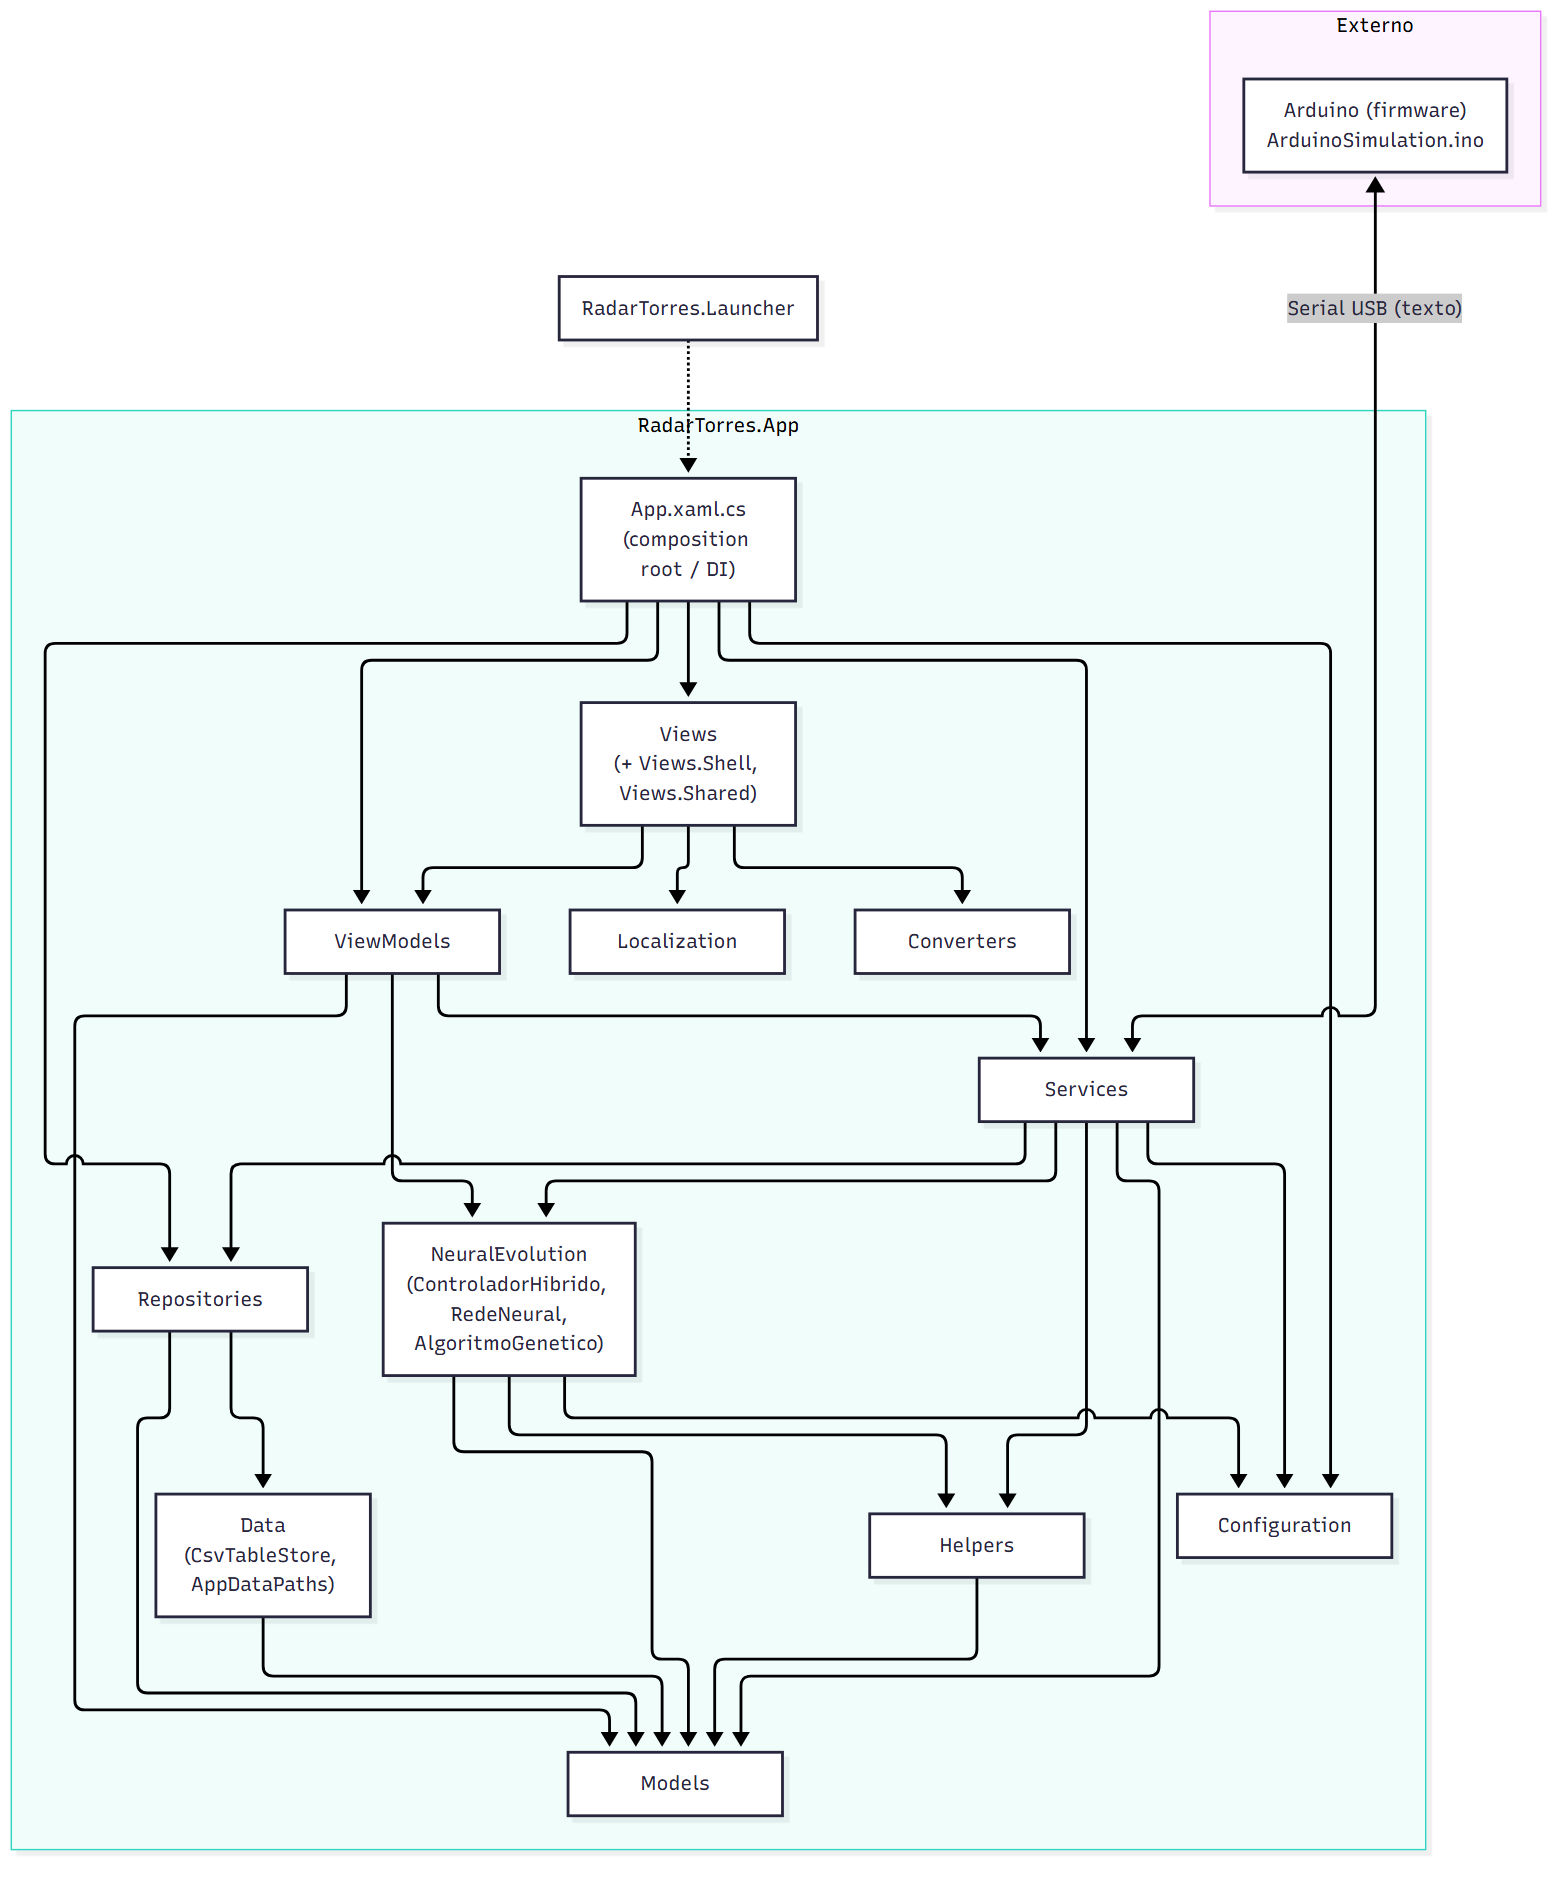
\includegraphics[width=0.8\textwidth]{Diagrama_de_Pacotes.png}
  \caption{Diagrama de pacotes do RadarTorres (dos autores).}
  \label{fig:pacotes}
\end{figure}

A extração a partir do código revelou dois ciclos de dependência, que a figura não destaca: o
serviço de navegação instancia telas (Services $\rightarrow$ Views, fechando o ciclo com Views
$\rightarrow$ ViewModels $\rightarrow$ Services), e o carregador de dados iniciais importa
repositórios e serviços (Data $\rightarrow$ Repositories/Services, fechando o ciclo com
Repositories/Services $\rightarrow$ Data). Como todos os pacotes estão no mesmo \textit{assembly},
os ciclos não impedem o funcionamento, mas aumentam o acoplamento e dificultam testes isolados.

% ------------------------------------------------------------
\subsection{Modelo de dados}
\label{sec:modelo-dados}

A persistência usa SQLite, banco embarcado em arquivo único, sem servidor e com chaves estrangeiras
habilitadas. A escolha é coerente com a implantação em nó único da Figura~\ref{fig:implantacao}:
nenhuma porta de rede exposta e nenhuma administração de servidor. O esquema tem onze tabelas
(Tabela~\ref{tab:tabelas-sqlite}): sete cadastrais e de auditoria, e quatro que persistem o histórico
do treinamento do controlador.

\begin{table}[H]
  \centering
  \caption{Tabelas do esquema SQLite.}
  \label{tab:tabelas-sqlite}
  \small
  \begin{tabularx}{\textwidth}{@{}lL@{}}
    \toprule
    \textbf{Tabela} & \textbf{Finalidade} \\
    \midrule
    \multicolumn{2}{@{}l}{\textit{Cadastro e auditoria}} \\
    Usuários & Contas, perfil (administrador, operador, visualizador) e autenticação \\
    Preferências do usuário & Tema, idioma e layout da interface por usuário \\
    Câmeras & Câmera responsável por cada quadrante \\
    Objetos detectados & Ocorrências de detecção por radar e câmera \\
    Estados da ocorrência & Transições de estado de cada ocorrência (só inserção) \\
    Classificações do alvo & Classificação de perigo pela velocidade estimada \\
    Ações realizadas & Acionamentos executados (só inserção) \\
    Modo atual da torre & Trocas de modo de operação (só inserção) \\
    \midrule
    \multicolumn{2}{@{}l}{\textit{Treinamento do controlador}} \\
    Histórico de gerações & \textit{Fitness} melhor e médio e alvos interceptados por geração \\
    Marcos de \textit{fitness} & Agregados por bloco de gerações \\
    Instantâneos do melhor indivíduo & Comportamento e genoma do melhor indivíduo em cada marco \\
    \bottomrule
  \end{tabularx}
\end{table}

A Figura~\ref{fig:der} mostra o núcleo de detecção e auditoria, a parte mais conectada do esquema.
As tabelas de treinamento são séries temporais independentes, sem chaves estrangeiras para as
demais. As tabelas de auditoria só aceitam inserção, de modo que o histórico de acionamentos e de
trocas de modo não pode ser alterado pela aplicação.

\begin{figure}[H]
  \centering
  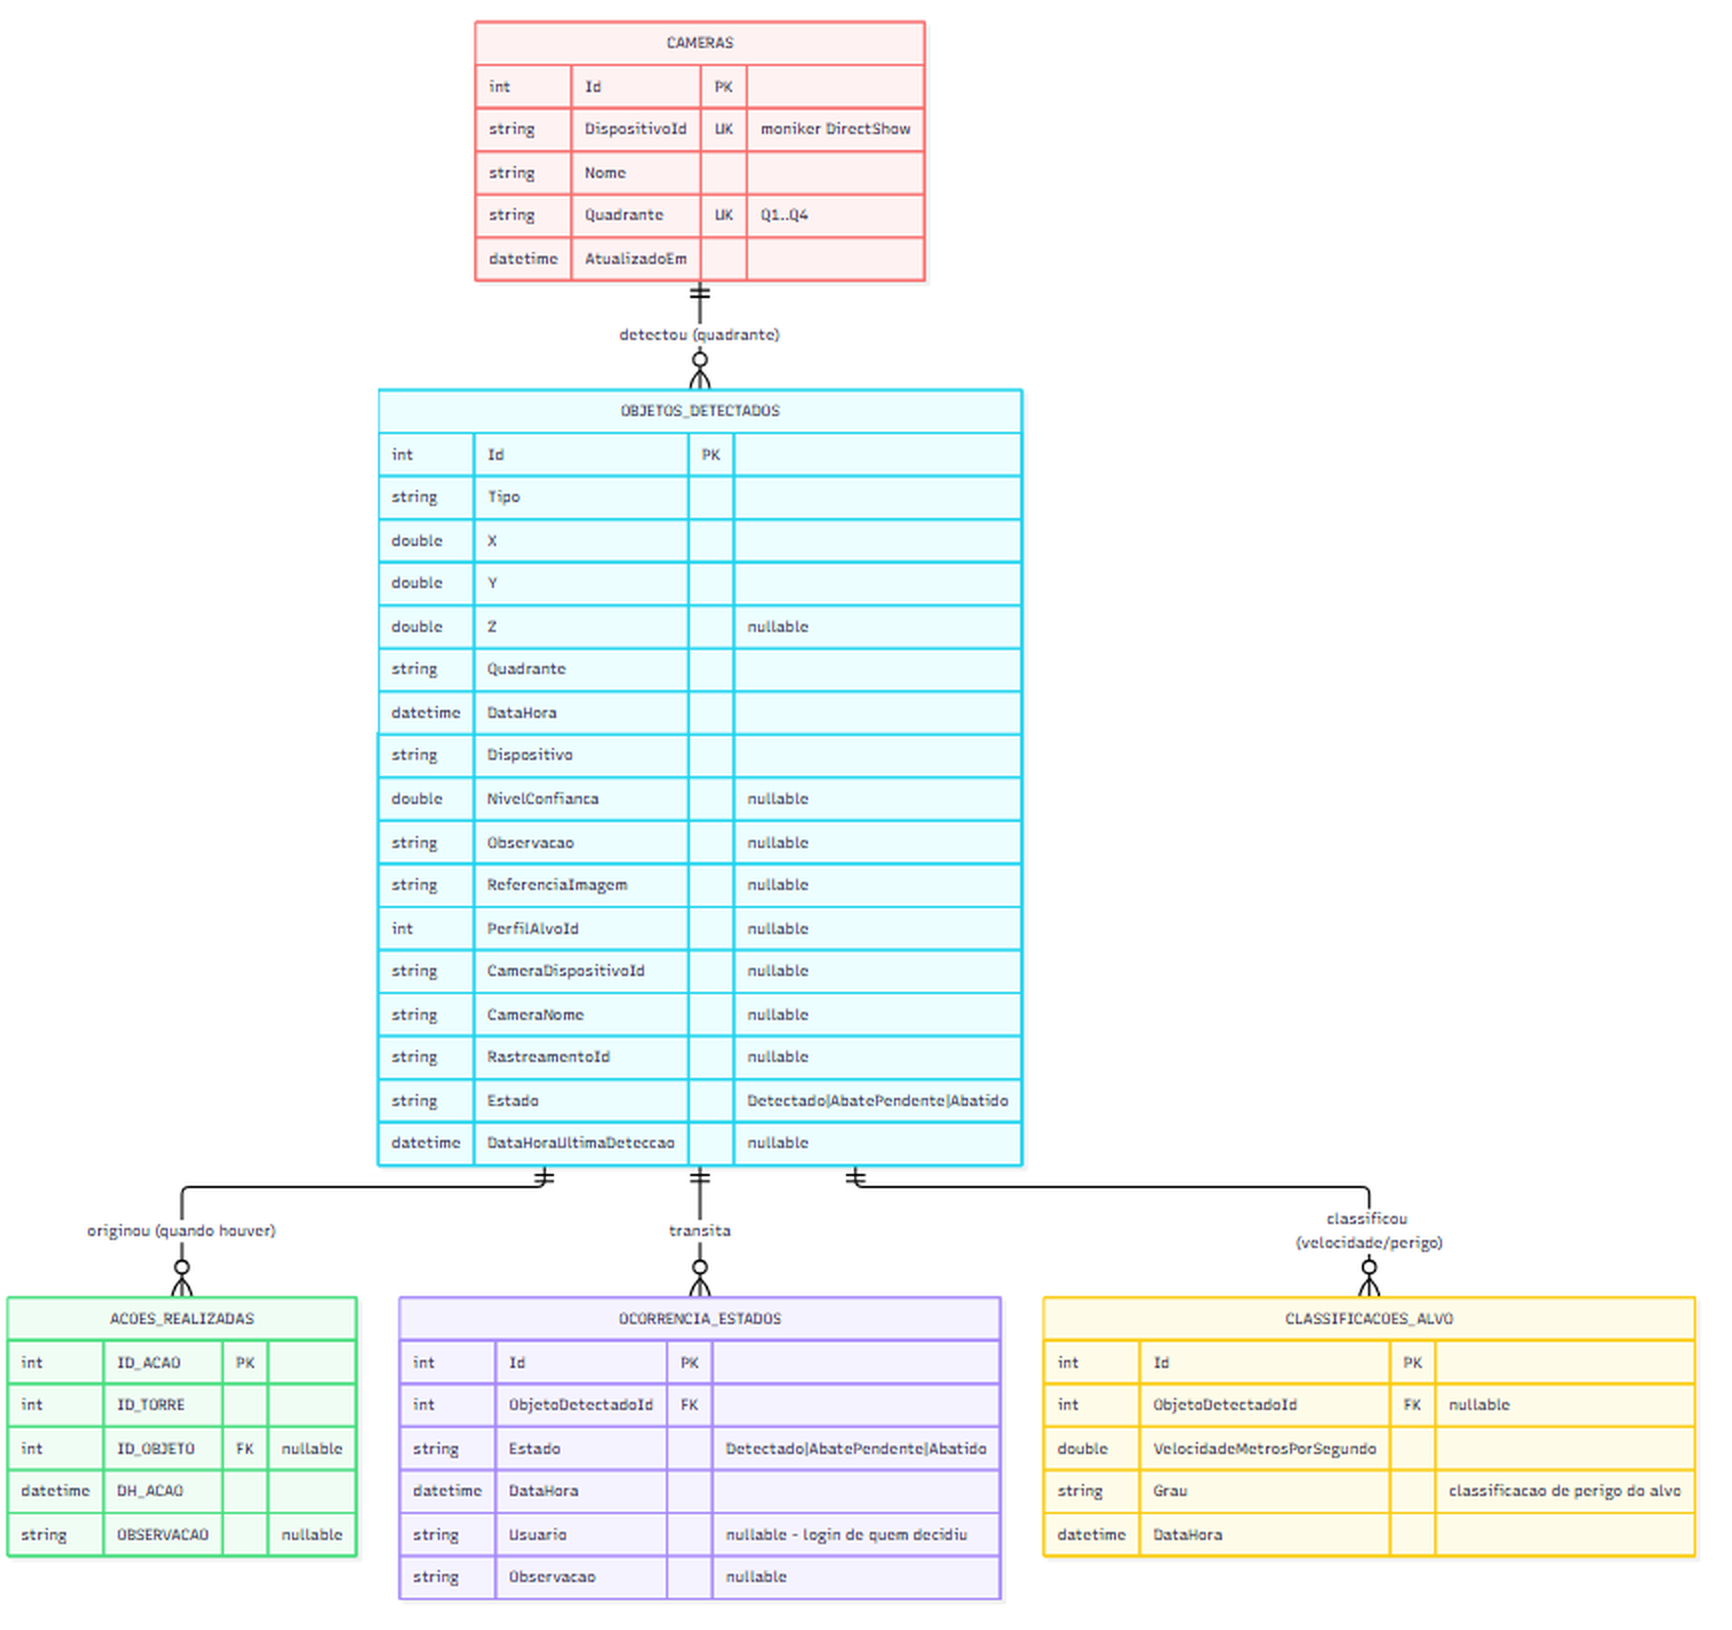
\includegraphics[width=0.6\textwidth]{DER_Cameras_Objetos_Detectados.png}
  \caption{Núcleo de detecção e auditoria do modelo de dados (dos autores).}
  \label{fig:der}
\end{figure}

% ------------------------------------------------------------
\subsection{Resultados e discussão}
\label{sec:resultados}

\subsubsection{Comparação pareada dos modos de decisão}

A Tabela~\ref{tab:comparacao} mostra o resultado do protocolo da Seção~\ref{sec:metodologia}. Para
cada modo treinável, a linha agregada usa, em cada seed de teste, a média das cinco execuções; as
diferenças são pareadas por seed em relação à heurística pura.

\begin{table}[H]
  \centering
  \caption{\textit{Fitness} em 200 seeds de teste reservadas. $\Delta$: diferença pareada em relação
  à heurística pura; $p$: teste de Wilcoxon pareado; M/P/I: seeds em que o modo foi melhor, pior ou
  igual à heurística.}
  \label{tab:comparacao}
  \small
  \begin{tabular}{@{}lrcrcrc@{}}
    \toprule
    \textbf{Modo} & \textbf{Média} & \textbf{IC95\%} & \textbf{$\Delta$} & \textbf{IC95\% de $\Delta$} & \textbf{$p$} & \textbf{M/P/I} \\
    \midrule
    Heurística pura & 120,49 & [110,1; 130,9] & -- & -- & -- & -- \\
    \midrule
    Híbrido, execuções 1 a 5$^{a}$ & 120,49 & [110,1; 130,9] & 0,00 & [0,0; 0,0] & 1,00 & 0/0/200 \\
    \midrule
    Rede pura, execução 1 & 121,82 & [111,7; 131,9] & $+$1,33 & [$-$7,8; 10,5] & 0,79 & 89/84/27 \\
    Rede pura, execução 2$^{b}$ & 117,68 & [107,8; 127,5] & $-$2,82 & [$-$12,0; 6,4] & 0,30 & 82/103/15 \\
    Rede pura, execução 3 & 120,53 & [110,8; 130,2] & $+$0,04 & [$-$8,9; 9,0] & 0,06 & 62/122/16 \\
    Rede pura, execução 5 & 115,58 & [105,3; 125,9] & $-$4,91 & [$-$15,9; 6,1] & 0,27 & 72/93/35 \\
    Rede pura, média das 5 & 118,66 & [109,9; 127,4] & $-$1,84 & [$-$10,1; 6,4] & 0,06 & -- \\
    \bottomrule
    \multicolumn{7}{@{}l}{\footnotesize $^{a}$ As cinco execuções produziram o mesmo resultado em todas as seeds.} \\
    \multicolumn{7}{@{}l}{\footnotesize $^{b}$ A execução 4 convergiu para o mesmo comportamento da execução 2 e teve resultado idêntico.}
  \end{tabular}
\end{table}

O desvio padrão do \textit{fitness} entre cenários é alto (cerca de 75 para uma média de 120): um
alvo que nasce em posição desfavorável pode invadir uma torre e encerrar o episódio, qualquer que
seja o controlador. É essa variância que torna necessária a comparação pareada; uma comparação
entre médias isoladas não distinguiria diferenças de alguns pontos.

O controlador híbrido produziu, nas cinco execuções, exatamente o mesmo \textit{fitness} que a
heurística pura em todas as 200 seeds, embora as redes evoluídas tenham topologias diferentes
(de 11 a 38 conexões). Nenhuma das 4631 oportunidades de acionamento foi recusada. A rede pura, sem
o filtro heurístico, mudou o resultado em 165 a 185 das 200 seeds, mas para melhor e para pior em
proporções parecidas: nenhuma execução diferiu significativamente da heurística ($p \geq 0{,}06$),
e a média das cinco ficou 1,84 ponto abaixo dela, com intervalo de confiança que inclui o zero.

Um detalhe do treinamento reforça a lição sobre seeds discutida adiante: o pico de \textit{fitness}
de treinamento ocorreu na geração 979 em todas as execuções do híbrido e na geração 334 em três das
cinco execuções da rede pura. O pico de treinamento reflete, em boa parte, a geração com cenários
mais fáceis, o que reforça a decisão de reportar apenas o desempenho nas seeds de teste.

\subsubsection{Falhas metodológicas encontradas no processo}

Antes do protocolo atual, o treinamento passou por três problemas que invalidavam silenciosamente
as conclusões e que só foram identificados ao investigar resultados inesperados. Eles são relatados
porque são o tipo de falha que métricas agregadas não revelam.

\textbf{Certeza de identificação estática.} Em uma versão anterior da simulação, a certeza de
identificação de cada alvo era sorteada uma única vez, no nascimento, e nunca atualizada; cerca de
70\% dos alvos nasciam abaixo do limiar de acionamento e nunca podiam ser interceptados. A
Tabela~\ref{tab:certeza} compara o histórico de treinamento antes e depois da correção, que passou a
fazer a certeza crescer com o tempo de observação. O efeito principal foi sobre a média da população,
que passou de cerca de 9 para cerca de 134; o melhor indivíduo variou bem menos (de cerca de 120
para cerca de 137, +15\%). A falha, portanto, não impedia que bons indivíduos surgissem, mas tornava
a média da população um indicador sem significado, que sugeria estagnação. Os dois períodos foram
registrados em versões diferentes do ambiente, de modo que a comparação é apenas indicativa.

\begin{table}[H]
  \centering
  \caption{\textit{Fitness} registrado no histórico de treinamento antes e depois da correção da
  certeza estática (versão anterior do ambiente).}
  \label{tab:certeza}
  \small
  \begin{tabular}{@{}lrr@{}}
    \toprule
    \textbf{Indicador} & \textbf{Antes} & \textbf{Depois} \\
    \midrule
    \textit{Fitness} médio da população & 9,11 & 134,17 \\
    Melhor \textit{fitness} por bloco de gerações & 119,62 & 137,35 \\
    Alvos que podiam ser acionados & $\approx$ 30\% & 100\% \\
    \bottomrule
  \end{tabular}
\end{table}

\textbf{Recusa aprendida de acionamento.} Na arquitetura anterior, uma rede de topologia fixa
evoluída por um algoritmo genético próprio, as redes treinadas recusavam entre 10\% e 56\% das
oportunidades legítimas de acionamento -- situações em que todos os vetos já haviam liberado e a
heurística pura acionaria --, e ficavam abaixo da heurística no \textit{fitness} médio. O
\textit{fitness} não tinha custo para a hesitação. Acrescentar uma penalidade de 3 pontos por recusa
levou a taxa de recusa a 0\%, e a rede passou a reproduzir a decisão de acionamento da heurística.
É por isso que a penalidade faz parte do \textit{fitness} atual e que a recusa é 0\% na
Tabela~\ref{tab:comparacao}.

\textbf{Grade de hiperparâmetros que media o sorteio de cenários.} Uma grade de onze configurações
(população de 30 a 120, 4 a 16 neurônios ocultos, mutação de 0,04 a 0,16), com uma execução cada,
terminou com o mesmo pico de \textit{fitness} (68,33 a 68,34) na mesma geração (222) em todas as
configurações. O resultado não indicava insensibilidade aos hiperparâmetros, e sim um defeito de
desenho: todas as configurações eram avaliadas, em cada geração, com as mesmas seeds, e o pico
registrava o maior \textit{fitness} já observado. Esse pico mede, portanto, a geração cujo sorteio
de cenários foi mais favorável. Para verificar a magnitude do efeito, um controlador fixo (a
heurística pura) foi avaliado nos conjuntos de seeds de 300 gerações: o \textit{fitness} variou de
33,9 a 119,8 (média 80,5; desvio padrão 13,9) apenas pela troca de cenários, uma variação maior do
que qualquer efeito de hiperparâmetro que a grade poderia detectar. A grade foi descartada, e a
configuração de produção não tem, hoje, justificativa experimental além de ser o padrão do sistema.
O protocolo atual corrige o defeito com avaliação final em seeds reservadas e várias execuções
independentes.

\subsubsection{Discussão}
\label{sec:discussao}

O resultado principal é negativo. Na configuração atual, com uma torre por quadrante, a rede neural
não altera nenhuma decisão do controlador híbrido. A causa é estrutural: a primeira camada da
heurística contém no máximo uma torre, de modo que a rede só tem escolha quando a torre do quadrante
está ocupada e há duas adjacentes livres; e, com a penalidade de recusa, a rede aprendeu a nunca
recusar o acionamento. Em outras palavras, a heurística decide quase tudo e a rede não tem espaço
para refinar. A garantia de pior caso da arquitetura -- a rede nunca leva o sistema a uma decisão
fora do que a heurística permite -- continua válida, mas o ganho esperado do aprendizado não se
confirmou.

O modo rede pura responde à segunda parte da pergunta de pesquisa. Sem a heurística, a rede
aprendeu uma política diferente, que muda o resultado na maioria dos cenários, mas não é melhor nem
significativamente pior: a camada heurística não é necessária para o desempenho médio, e sim para a
previsibilidade, já que só com ela é possível garantir que nenhuma torre fora do quadrante seja
escolhida sem motivo. Em uma versão anterior do ambiente, um genoma em modo rede pura chegou a
superar o híbrido e a heurística, sem teste estatístico; esse resultado não se reproduziu com o
protocolo atual.

Três ressalvas limitam o alcance dessas conclusões. Primeiro, a simulação não é calibrada: a curva
de crescimento da certeza, a probabilidade de erro e as trajetórias são premissas, e o ambiente
simulado é maior e mais rápido do que o sensoriamento físico permitiria
(Seção~\ref{sec:hardware}). Segundo, há uma diferença entre simulação e produção: na simulação, o
modo híbrido consulta a confiança de acionamento da rede e impõe 0,3~s de mira; em produção, o
acionamento depende só do veto heurístico. Como a rede treinada nunca recusa, a diferença não altera
o comportamento observado, mas deveria ser eliminada. Terceiro, o SharpNEAT não recebe uma semente
fixa, então as execuções de treinamento são réplicas independentes, mas não reproduzíveis bit a bit;
os cenários de teste, ao contrário, são reproduzíveis pela seed.

% ============================================================
% 3 CONCLUSÃO
% ============================================================
\section{Conclusão}

Este trabalho apresentou o RadarTorres, protótipo de software que simula, com sensores
ultrassônicos e câmeras, a cadeia de detecção, localização e seleção de torres de um sistema de
defesa, e que decide por meio de um controlador híbrido -- heurística determinística que filtra e
veta, rede neural evoluída por NEAT que ajusta a priorização. Foram implementados a aquisição e o
protocolo serial, o radar, a detecção visual, o controlador, o ambiente de treinamento, a auditoria
e o controle de acesso, e documentadas a implantação, a arquitetura de pacotes e o modelo de dados.

A resposta à pergunta de pesquisa é negativa para a configuração estudada. Avaliado em 200 cenários
de teste reservados, com cinco execuções independentes e teste de Wilcoxon pareado, o controlador
híbrido foi idêntico à heurística pura, e a rede pura não diferiu significativamente dela. A
arquitetura híbrida cumpre a função de limitar o pior caso, mas, com uma torre por quadrante, a
heurística deixa à rede um espaço de decisão praticamente vazio. O resultado não mostra que a
neuroevolução seja inútil para o problema; mostra que, para ela acrescentar algo, o problema precisa
oferecer escolhas que a heurística não resolve.

O processo também produziu lições metodológicas: uma premissa errada da simulação (a certeza
estática) mascarou a evolução sob aparência de estagnação; um \textit{fitness} sem custo para a
hesitação ensinou a rede a recusar acionamentos; e uma grade de hiperparâmetros com seeds
compartilhadas mediu o sorteio de cenários, e não as configurações. Cada uma passaria despercebida se
o trabalho reportasse apenas o melhor \textit{fitness} de treinamento.

As limitações principais são a ausência de validação física e de calibração da simulação, a falta de
avaliação quantitativa da visão computacional e a distância entre os parâmetros simulados e o que o
sensoriamento ultrassônico permite. Como trabalhos futuros, propõem-se: (i) um ensaio de bancada do
HC-SR04 sobre o motor de varredura, para calibrar o modelo de ruído da simulação; (ii) a avaliação
da visão com um conjunto de imagens rotulado, medindo acurácia e taxa de quadros; (iii) cenários com
mais de uma torre por quadrante, ou com escolhas de alocação entre vários alvos, em que a rede tenha
espaço para refinar a heurística; (iv) a abordagem multiameaça da literatura de TEWA; (v) a fusão
entre câmera e ultrassom; e (vi) a substituição do ultrassom por um radar real, evolução natural de
um sistema cujo sensoriamento foi desenhado para simulá-lo.

% ============================================================
% REFERÊNCIAS
% ============================================================
\bibliography{referencias}

\end{document}
